% Trabalho Academico FATEC-SJC v-1.1
% Criado por Marcos Hideki Inoue Junior

% -- Iniciando o documento --
\documentclass[
	12pt,		% Tamanho da fonte
	a4paper,	% Tamanho do papel
	english,	% Idioma adicional
	brazil,		% Idioma principal
	openright,	% Capitulos começam em pag impar
	oneside		% Apenas 1 página por folha
	]{abntex2}

\usepackage{lmodern}			% Usa a fonte Latin Modern
\usepackage[T1]{fontenc}		% Selecao de codigos de fonte.
\usepackage[utf8]{inputenc}		% Codificacao do documento
\usepackage{lastpage}			% Usado pela Ficha catalográfica
\usepackage{indentfirst}		% Indenta o primeiro parágrafo de cada seção.
\usepackage{color}				% Controle das cores
\usepackage{xcolor}
\usepackage{graphicx}			% Inclusão de gráficos
\usepackage{microtype} 			% para melhorias de justificação
\usepackage{lipsum}				% para geração de dummy text
\usepackage{geometry}			% para alteração no layout das páginas
\usepackage{lscape}             % colocar páginas na horizontal compativel com longtable e supertabular.
\usepackage{bookmark}
\usepackage{caption}            % adiciona \caption*{d} para criar fontes em imagens.
\usepackage{float}				% para uso no posicionamento de imagens
\usepackage{pdfpages}
\usepackage{minibox}
\usepackage{listings}
\usepackage{multirow}           % Habilita o Merge de celulas na table

% ---
% Alterações no modelo original da abnTex2
% ---
% Impressão da Capa
\renewcommand{\imprimircapa}{%
  \begin{capa}%
    \center
    \ABNTEXchapterfont\large\imprimirinstituicao\\
    \vspace{5cm}
    \imprimirautor

    \vfill
    \begin{center}
    \ABNTEXchapterfont\bfseries\LARGE\imprimirtitulo
    \end{center}
    \vfill

    \large\imprimirlocal

    \large\imprimirdata

    \vspace*{1cm}
  \end{capa}
}
% ---
% Alteração na assinatura dos componentes da banca
\setlength{\ABNTEXsignwidth}{10cm}

\geometry{
 a4paper,
 bottom=2cm,
 top=3cm,
 left=3cm,
 right=2cm
}

% ---
% Configura layout para elementos textuais
\renewcommand{\textual}{%
  \pagestyle{plain}%abntheadings
  %\nouppercaseheads%
  \bookmarksetup{startatroot}%
  \pagenumbering{arabic}
}

\renewcommand{\pretextual}{%
  \pagestyle{plain}
  \pagenumbering{Roman}
}

%%% -----
%%% Formato de cabeçalho/rodapé romano nos elementos pré-textuais
%%% -----

%% Novo estilo
\makepagestyle{estilo_pretextual} %%% escolha um nome
  %\makeevenhead{estilo_pretextual}{}{}{\ABNTEXfontereduzida \textbf \thepage}
  \makeoddhead{estilo_pretextual}{}{}{\ABNTEXfontereduzida \textbf \thepage}

%% Customiza comando \pretextual
\renewcommand{\pretextual}{
  \pagenumbering{Roman} %%% ou \pagenumbering{Roman}
  \aliaspagestyle{chapter}{estilo_pretextual}% customizing chapter pagestyle
  \pagestyle{estilo_pretextual}
  \aliaspagestyle{cleared}{empty}
  \aliaspagestyle{part}{estilo_pretextual}
}

% ---
% Ajusta a marca \textual para que a numeração volte a ser arábica
% nos elementos textuais
\let\oldtextual\textual        % copia o comando \textual anterior para \oldtextual
\renewcommand{\textual}{%
  \pagestyle{plain}%abntheadings
  %\nouppercaseheads%
  \aliaspagestyle{chapter}{plain}
  \bookmarksetup{startatroot}%
  \pagenumbering{arabic}
}
% ---

\makeatletter
\renewcommand*{\ps@plain}{%
  \let\@mkboth\@gobbletwo
  \let\@oddhead\@empty
  \def\@oddfoot{%
    \reset@font
    \hfil
    \thepage
    % \hfil % removed for aligning to the right
  }%
  \let\@evenhead\@empty
  \let\@evenfoot\@oddfoot
}
\makeatother

% ---
% Pacotes de citações
% ---
\usepackage[brazilian, hyperpageref]{backref}	 % Paginas com as citações na bibl
\usepackage[alf]{abntex2cite}	% Citações padrão ABNT



% ---
% CONFIGURAÇÕES DE PACOTES
% ---

% ---
% Configurações do pacote backref
% Usado sem a opção hyperpageref de backref
\renewcommand{\backrefpagesname}{Citado na(s) página(s):~}
% Texto padrão antes do número das páginas
\renewcommand{\backref}{}
% Define os textos da citação
\renewcommand*{\backrefalt}[4]{
	\ifcase #1 %
		Nenhuma citação no texto.%
	\or
		Citado na página #2.%
	\else
		Citado #1 vezes nas páginas #2.%
	\fi}%
% ---

% ---
% Informações de dados para CAPA e FOLHA DE ROSTO
% ---
\titulo{Titulo do TG}

\autor{Nome Completo do Autor}
\local{São José dos Campos}
\data{\the\year}

\orientador{TituloDoOrientador. Nome do Orientador}
\coorientador{TituloDoCoorientador. Nome do coorientador}

\instituicao{%
  FACULDADE DE TECNOLOGIA DE SÃO JOSÉ DOS CAMPOS
  \par
  FATEC PROFESSOR JESSEN VIDAL}

\tipotrabalho{Trabalho de Graduação}

\newcommand{\disciplina}{Banco de Dados}

\preambulo{Trabalho de Graduação apresentado à Faculdade de Tecnologia São José dos Campos, como parte dos requisitos necessários para a obtenção do título de Tecnólogo em \disciplina.}

% Comandos para a folha de catalogacao
\newcommand{\cursoRef}{Curso de Tecnologia em Banco de Dados}
\newcommand{\instituicaoRef}{FATEC de S\~ao Jos\'e dos Campos: Professor Jessen Vidal}
\newcommand{\sobrenomeRef}{SobrenomeReferencia}
\newcommand{\nomeRef}{nomesReferencia}
\newcommand{\rgRef}{12.345.678-9}
% informações do PDF
\makeatletter
\hypersetup{
     	%pagebackref=true,
		pdftitle={\@title},
		pdfauthor={\@author},
    	pdfsubject={\imprimirpreambulo},
	    pdfcreator={LaTeX with abnTeX2},
		pdfkeywords={abnt}{latex}{abntex}{abntex2}{trabalho acadêmico},
		colorlinks=true,       		% false: boxed links; true: colored links
    	linkcolor=blue,          	% color of internal links
    	citecolor=blue,        		% color of links to bibliography
    	filecolor=magenta,      		% color of file links
		urlcolor=blue,
		bookmarksdepth=4
}
\makeatother

% ---
% Espaçamentos entre linhas e parágrafos
% ---
\setlength{\parindent}{1.3cm} % Tamanho do parágrafo

% Controle do espaçamento entre um parágrafo e outro:
\setlength{\parskip}{0.2cm}  % tente também \onelineskip

% ---
% compila o indice
% ---
\makeindex
% ---

% ----
% Início do documento
% ----
\begin{document}
\pretextual
\selectlanguage{brazil}
\frenchspacing % Retira espaço extra obsoleto entre as frases

% ---
% Configuring all citations
\citeoption{abnt-etal-list=0}
\citeoption{abnt-last-names=abnt}
\citeoption{abnt-full-initials=yes}
% ---

% ---
% Configuring listing code
% See references on internet
% ---
\lstdefinestyle{customc}{
  belowcaptionskip=1\baselineskip,
  breaklines=true,
  %frame=L,
  xleftmargin=\parindent,
  language=C,
  numbers=left,
  showstringspaces=false,
  frame=single,
  basicstyle=\footnotesize\ttfamily,
  keywordstyle=\bfseries\color{green!40!black},
  commentstyle=\itshape\color{purple!40!black},
  identifierstyle=\color{blue},
  stringstyle=\color{orange},
}

\lstset{escapechar=@,style=customc}

% ---

% ---
% Capa
% ---
\imprimircapa
% ---

% ---
% Folha de rosto
% (o * indica que haverá a ficha bibliográfica)
% ---
\thispagestyle{empty}
\imprimirfolhaderosto
% ---

% ---
% Inserir a ficha bibliografica
% ---

\begin{fichacatalografica}
    %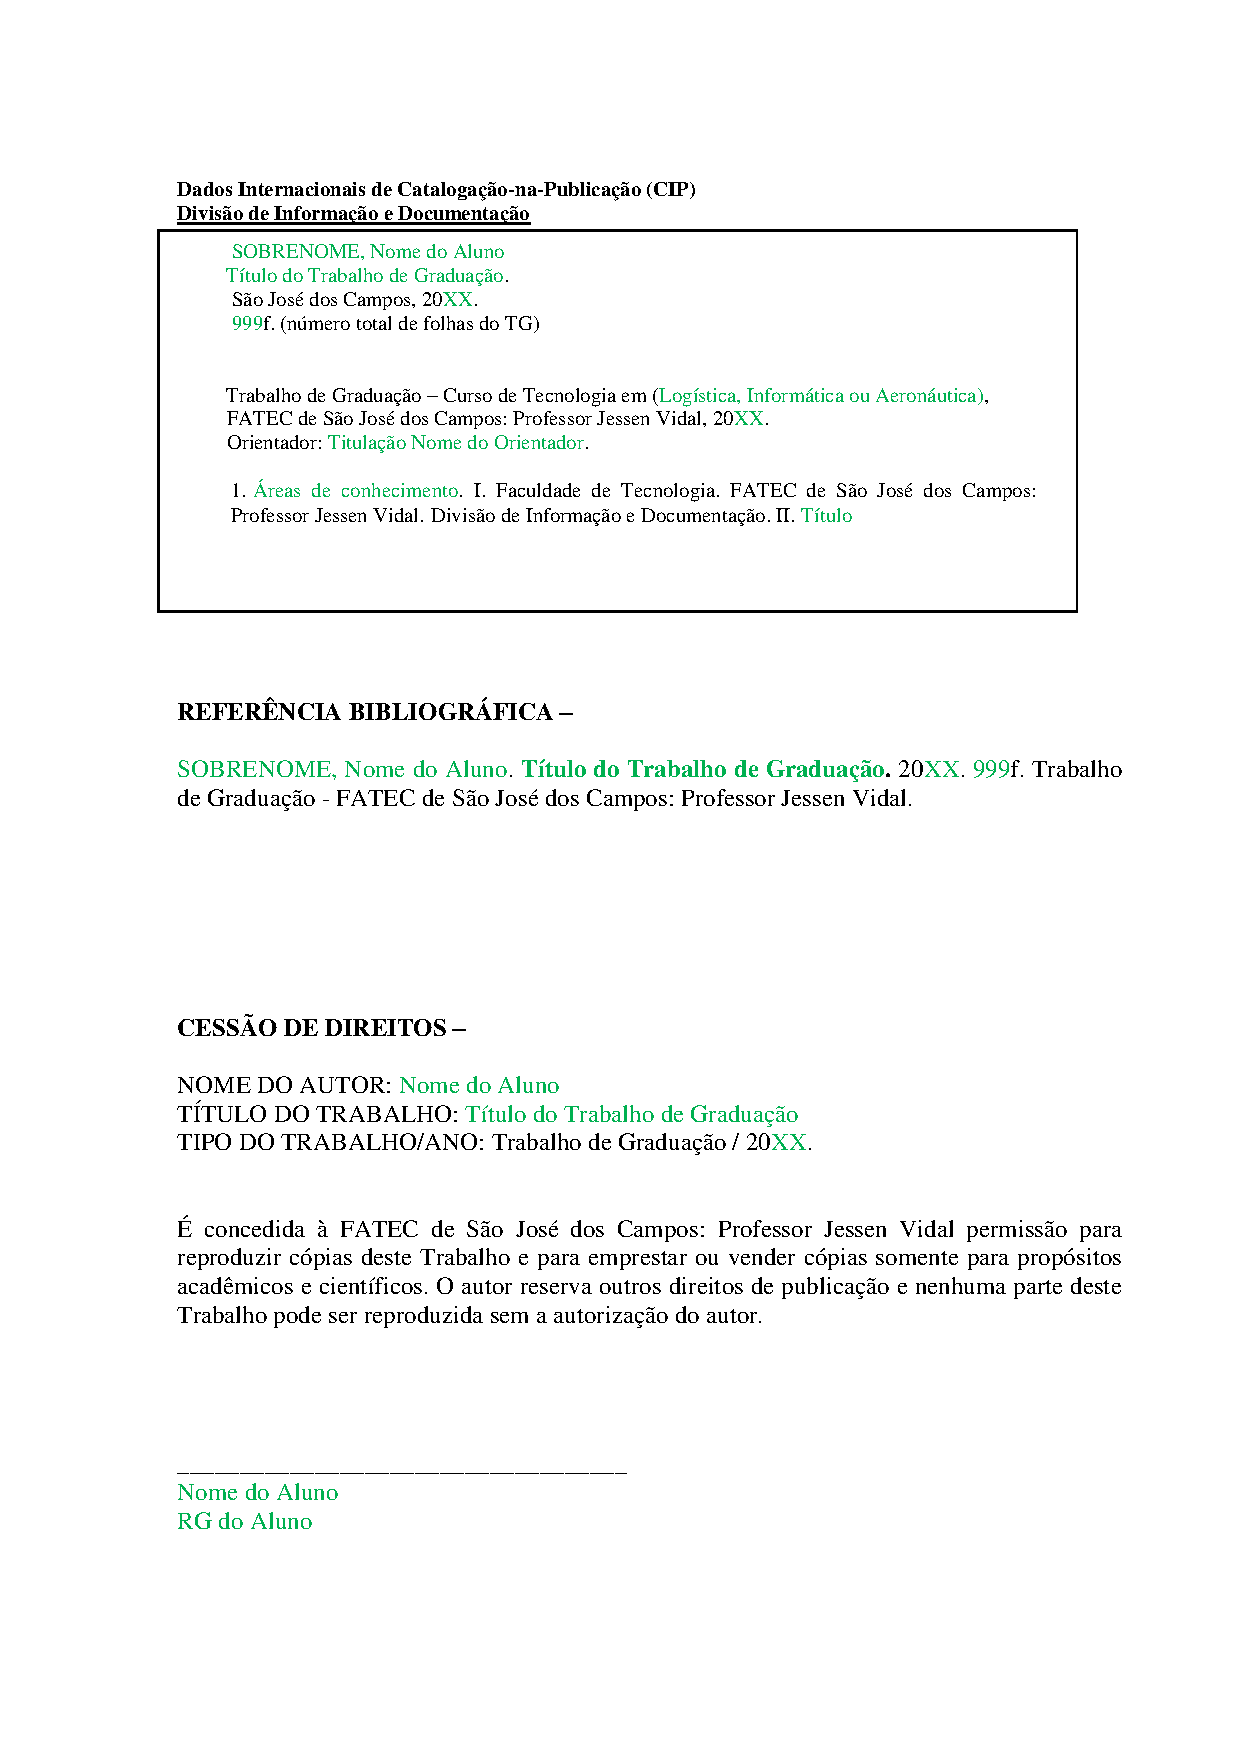
\includepdf{./testFicha}
    %%%%%%%%%%%%%
%
% Do not Edit this file!
%
%%%%%%%%%%%%%

\noindent\textbf{Dados Internacionais de Catalogação-na-Publicação (CIP)\\
Divisão de Informação e Documentação}

%\noindent\minibox[frame]{%
%    \indent INOUE, Marcos Hideki \\
%    \indent \imprimirtitulo \\
%    \indent \imprimirlocal, \the\year \\
%    \indent \pageref{LastPage}f. \\
%    \\ \\
%    \indent \imprimirtipotrabalho \-m \cursoRef \\
%    \indent \instituicaoRef, \the\year \\
%    \indent Orientador: \imprimirorientador \\
%    \indent Coorientador: \imprimircoorientador \\
%    \\
%    \indent \'Areas de Conhecimento. I. Faculdade de Tecnologia. \instituicaoRef. Divis\~ao de Informa\c{c}\~ao e Documenta\c{c}\~ao. II. \imprimirtitulo.
%}%

\noindent\framebox[\textwidth]{%
  % horizonal margin: 10\unitlength
  \parbox{400\unitlength}{%
    \sobrenomeRef, \nomeRef \\
    \imprimirtitulo \\
    \imprimirlocal, \the\year \\
    \pageref{LastPage}f. \\
    \\ \\
    \imprimirtipotrabalho\ -- \cursoRef \\
    \instituicaoRef, \the\year \\
    Orientador: \imprimirorientador \\
    Coorientador: \imprimircoorientador \\
    \\
    \'Areas de Conhecimento. I. Faculdade de Tecnologia. \instituicaoRef. Divis\~ao de Informa\c{c}\~ao e Documenta\c{c}\~ao. II. \imprimirtitulo
  }%
}\\
\parbox{400\unitlength}{
\vspace*{2cm}

\textbf{REFER\^ENCIA BIBLIGR\'AFICA ---} \\ \\
\sobrenomeRef, \nomeRef. \imprimirtitulo \the\year. \pageref{LastPage}f. \imprimirtipotrabalho\ -- \instituicaoRef.

\vspace*{3cm}
\textbf{CESS\~AO DE DIREITOS ---}\\ \\
NOME DO AUTOR: \imprimirautor \\
T\'ITULO DO TRABALHO: \imprimirtitulo \\
TIPO DO TRABALHO/ANO: \imprimirtipotrabalho/\the\year \\

\vspace*{2cm}
É concedida à FATEC de São José dos Campos: Professor Jessen Vidal permissão para reproduzir cópias deste Trabalho e para emprestar ou vender cópias somente para propósitos acadêmicos e científicos. O autor reserva outros direitos de publicação e nenhuma parte deste Trabalho pode ser reproduzida sem a autorização do autor.\\

\vspace*{2cm}
\noindent\rule{7cm}{0.4pt}\\
\imprimirautor \\RG: \rgRef
}
\end{fichacatalografica}

% ---
% Folha de aprovação
% ---

% Descomentar para imprimir a folha
\begin{folhadeaprovacao}

  \begin{center}
    {\ABNTEXchapterfont\large\imprimirautor}

    \vspace*{\fill}\vspace*{\fill}
    \begin{center}
      \ABNTEXchapterfont\bfseries\Large\imprimirtitulo
    \end{center}
    \vspace*{\fill}

    \hspace{.45\textwidth}
    \begin{minipage}{.5\textwidth}
        \imprimirpreambulo
    \end{minipage}%
    \vspace*{\fill}

    Composição da Banca
   \end{center}

   \assinatura{\textbf{\imprimirorientador} \\ Orientador\\}
   \begin{center}
   {\textbf{\imprimircoorientador} \\ Coorientador\\\vspace*{0.5cm}}
   {\textbf{Nome do Professor 1} \\ Professor Convidado\\\vspace*{0.5cm}}
   {\textbf{Nome do Professor 2} \\ Professor Convidado\\\vspace*{0.5cm}}
   %\assinatura{\textbf{Professor} \\ Convidado 4}
   % Adicionar \assinatura para inserir linha de assinatura dos professores convidados
\end{center}   
   \begin{center}
    \vspace*{0.5cm}
    {\large\imprimirlocal}
    \par
    {\large\imprimirdata}
    \vspace*{1cm}
  \end{center}

\end{folhadeaprovacao}

% Descomentar quando o arquivo folhaAprov.pdf estiver no diretorio raiz
%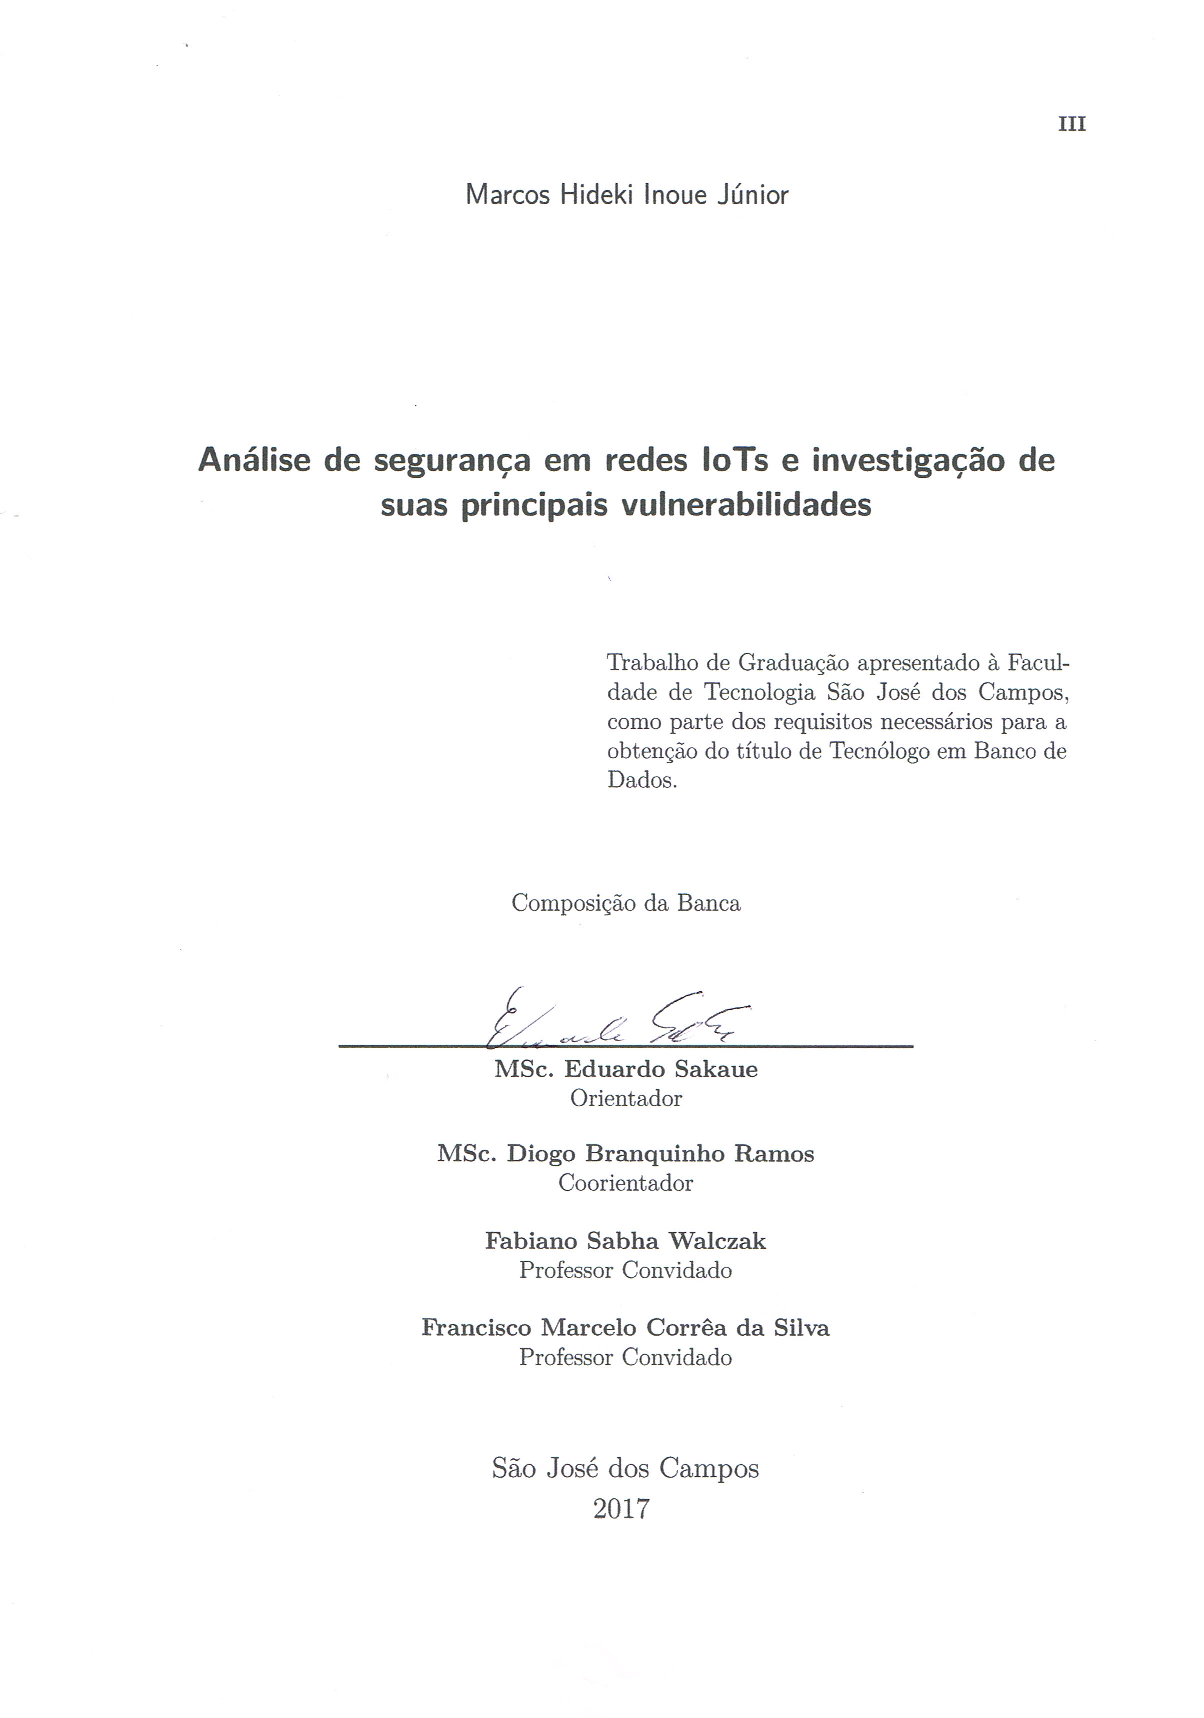
\includepdf[]{folhaAprov.pdf}
% ---

% ---
% Dedicatória
% ---
\begin{dedicatoria}
   \vspace*{\fill}
   \centering
   \noindent
   \textit{A todos aqueles que de alguma forma estiveram e est\~ao pr\'oximos de mim,\\ fazendo com que eu tenha DETERMINA\c{C}\~AO.}
   %\textit{Nós não conseguimos o que merecemos,\\ só conseguimos o que é possível.} 
   \vspace*{\fill}
\end{dedicatoria}
% ---

% ---
% Agradecimentos
% ---
\begin{agradecimentos}
\par Sou grato aos meus pais por tudo que fizeram e fazem por mim.
\par Agrade\c{c}o a Faculdade de Tecnologia de S\~ao Jos\'e dos Campos (FATEC-SJC) pela oportunidade de estudar nesta institui\c{c}\~ao de ensino maravilhosa que me proporcionou uma quantidade imensur\'avel de conhecimento.

\par Agrade\c{c}o tamb\'em o Instituto Nacional de Pesquisas Espaciais (INPE) pela oportunidade de est\'agio que me proporcionou muitas oportunidades para aumentar meu conhecimento e aprender sobre assuntos variados e a utiliza\c{c}\~ao de linguagens diferentes.

\par Agrade\c{c}o a microempresa Tecnologias para a Sustentabilidade (TecSUS) pela oportunidade de est\'agio e em conjunto com a mesma, sou grato \`a Microchip Technology e ao Ricardo Seiti da utiliza\c{c}\~ao de seus equipamentos e microcontroladores para a realiza\c{c}\~ao deste trabalho.

\par Sou extremamente grato tamb\'em ao meu orientador Eduardo Sakaue por sua orienta\c{c}\~ao, aten\c{c}\~ao e ajuda como orientador e como amigo. Tamb\'em ao meu coorientador Diogo Branquinho Ramos por sua coorienta\c{c}\~ao e ajuda seja como coorientador ou amigo.

\par Sou muito grato pelos meus professores que tive, em especial o professor Giuliano Bertoti que me motivou a realizar o modelo de \LaTeX, ao professor Emanuel Mineda por sua ajuda e amizade, ao professor Fabiano Sabha pela sua companhia e amizade e Jean Carlos pela sua amizade e companheirismo.

\par Sou muito agradecido pela companhia e amizade de minha melhor amiga Deborah Susan e de meus amigos e amigas: Safire Lauene, Samantha Marques, Camilo Damaso, William Siqueira, Erivan Lima, Luana C\^amara, Rafael Viana, Leonardo Neves, Pedro Valentim, Matheus Monteiro, Vanilson Leite, Reginaldo Moreira, Antônio Siqueira e Clélio Henrique.

\par Sou grato aos meus colegas de trabalho da TecSUS: Thiago Gomes, Wagner Fukuoka e Ariadne Mioni que me oferecem um \'otimo ambiente de trabalho. Tamb\'em agrade\c{c}o meus colegas de trabalho do INPE: Ver\^onica Maria, Rodrigo Takeshi, Anna Karina, M\"uller Lopes e Jos\'e Marchezi que me proporcionaram um ambiente de trabalho descontra\'ido e divertido, tamb\'em me incentivaram e me ajudaram com o uso do \LaTeX\ para a realiza\c{c}\~ao deste trabalho e a cria\c{c}\~ao do modelo de Trabalho de Gradua\c{c}\~ao para a FATEC-SJC utilizando \LaTeX.

\end{agradecimentos}
% ---

% ---
% Epigrafe
% ---
\begin{epigrafe}
    \vspace*{\fill}
    \begin{flushright}
% Little easter egg. 
%        \textit{''Eu acredito que os HotDogs simbolizam uma filosofia muito profunda, \\
%                na qual todos nós poderíamos ter a oportunidade de observá-la e aprendê-la. \\
%                O pão pode significar tudo que dá a nossa base para a nossa vida. \\
%                E a salsicha pode simbolizar nós mesmos, ou um simples conceito ou coisa que surge de uma epifania.''\\
%                (Rodrigo Takeshi, 26 de Outubro de 2016)}

        \textit{“Epigrafe, citar alguma frase de outra pessoa que tenha rela\~c\~ao com o TG”\\
        (Marcos Hideki)}
    \end{flushright}
\end{epigrafe}
% ---

% ---
% RESUMOS
% ---
% resumo em português
\setlength{\absparsep}{18pt} % ajusta o espaçamento dos parágrafos do resumo
% --- resumo em português ---
\begin{resumo}
    Apresentação concisa dos pontos relevantes do documento deve ser exposta no resumo. No presente caso o resumo será informativo, assim deverá ressaltar o objetivo, a metodologia, os resultados e as conclusões do documento. A ordem desses itens depende do tratamento que cada item recebe no documento original. O resumo deve ser composto por uma seqüência de frases concisas, afirmativas e não em enumeração de tópicos. Deve ser escrita em parágrafo único e espacejamento de 1,5. A primeira frase deve ser significativa, explicando o tema principal do documento. Deve-se usar o verbo na voz ativa e na terceira pessoa do singular. Quanto a sua extensão, o resumo deve possuir de 150 a 500 palavras.   
    \vspace{\onelineskip}
    \noindent
    \textbf{Palavras-chave}: palavras chaves, resumo, português.
\end{resumo}

% resumo em inglês
\begin{resumo}[Abstract]
    \begin{otherlanguage*}{english}
        O abstract é o resumo da obra em língua estrangeira, que basicamente segue o mesmo conceito e as mesmas regras que o texto em português. Recomenda-se que para o texto do abstract o autor traduza a versão do resumo em português e faça, se necessário, os ajustes referentes à conversão dos idiomas. É importante observar que o título e texto NÃO DEVEM estar em itálico.
	    \vspace{\onelineskip}
	    \noindent
	    \\
	    \textbf{Keywords}: Keywords, abstract, english.
    \end{otherlanguage*}
\end{resumo}
% ---

% ---
% inserir lista de ilustrações
% ---
\pdfbookmark[0]{\listfigurename}{lof}
\listoffigures*
\cleardoublepage
% ---

% ---
% inserir lista de tabelas
% ---
\pdfbookmark[0]{\listtablename}{lot}
\listoftables*
\cleardoublepage
% ---

% ---
% inserir lista de abreviaturas e siglas
% ---
% Listas de Siglas utilizadas no TG
\begin{siglas}
    \item[FaTeX] \emph{Fatec LaTeX}
    \item[TG] \emph{Trabalho de Gradua\~c\~ao}
\end{siglas}
% ---

% ---
% inserir lista de símbolos
% ---
% Lista de simbolos utilizadas no TG
\begin{simbolos}
  \item[$ m^2 $] Metro quadrado
  \item[GHz] Giga-hertz
  \item[MHz] Mega-hertz
\end{simbolos}
% ---
% ---
% inserir o sumario
% ---
\pdfbookmark[0]{\contentsname}{toc}
\tableofcontents*
\cleardoublepage
% ---

% ----------------------------------------------------------
% ELEMENTOS TEXTUAIS
% ----------------------------------------------------------

\textual

\setcounter{page}{15}
% ---
% Incluindo Capitulo 1 - Introducao
% ---
% ----------------------------------------------------------
% Introdução (exemplo de capítulo sem numeração, mas presente no Sumário)
% ----------------------------------------------------------
\chapter[Introdução]{Introdução}
%\addcontentsline{toc}{chapter}{Introdução}
% ----------------------------------------------------------
\par A maior parte da vida moderna depende dos computadores, das redes de computadores e atualmente a mais notável interação do ser humano é o deslizar do dedo em uma \emph{smartphone}. Essas tecnologias tendem a se integrar ainda mais com a nossa realidade com o avan\c{c}o tecnol\'ogico dos microcomputadores e microcontroladores, tornando assim o termo \emph{Internet of Things} (\emph{IoT}) cada vez mais conhecido pela sua peculiaridade de objetos se conectando \`a internet.

\par \emph{IoT} não é uma tecnologia nova, entretanto tem ganho maior espa\c{c}o com a necessidade das pessoas de receberem informa\c{c}\~oes sobre diversas coisas do seu dia a dia em tempo real, logo o termo significa nada mais do que objetos que realizam a\c{c}\~oes ou geram informa\c{c}\~oes conectados \`a internet. A principal ideia de \emph{IoT} vem da presença de coisas ou objetos de nosso dia a dia que são capazes de interagir e cooperar entre eles a fim de alcançar um objetivo em comum. A principal força da \emph{Internet of Things} vem da ideia na qual a mesma terá um grande impacto em diversos aspectos de nosso dia a dia e no comportamento de seus usuários, já que diversos cenários serão afetados por ela, como por exemplo o recebimento de informa\c{c}\~oes em tempo real de hidr\^ometros, monitoramento de vazamentos e entre diversos outros, com todas essas informa\c{c}\~oes dispon\'iveis na nuvem \'e poss\'ivel acess\'a-las de diversas maneiras, seja ela por um computador ou um \emph{smartphone}. Há diversas definições parecidas de \emph{IoT}, e atualmente muitas pessoas tem dificuldades para entender realmente o que significa seu conceito, suas ideias básicas e suas implicações sociais, econômicas e técnicas \cite{iot2005itu}.

\par Segundo \citeonline{Atzori2010a}, o que gera confus\~ao com o termo \emph{IoT} é o termo em sí, que une \emph{Internet} e \emph{Things}, dando uma ideia de conectividade que une coisas ou objetos. Expressa uma ideia genérica de objetos onde todos eles est\~ao unidos por um meio em comum, todavia há pequenas diferenças nos pontos de vista dos componentes da \emph{IoT}. O cenário como pode ser visto na \autoref{fig:iot} é dividido em 3 visões:
\begin{itemize}
    \item Visão orientada aos objetos, que são objetos do nosso dia a dia, como sensores, cart\~oes de \emph{Radio-Frequency Identification (RFID)} e entre outros.
    \item Visão orientada a Internet, trata da visão das redes ou da internet em si no contexto de \emph{IoT}, pode ser chamada de \emph{web} das coisas.
    \item Visão orientada a Semântica, visa os conceitos tecnol\'ogicos e te\'oricos em si.
\end{itemize}
Todas essas vis\~oes tornam as aplicações de \emph{IoT} muito abrangentes possibilitando uma variedade enorme de sistemas que poderão ser desenvolvidos. As principais atuações em nossas vidas estão em casa \emph{(Smart Home)} e em cidades \emph{(Smart Cities)}. São diversos domínios nas aplicações dessa tecnologia, e elas são agrupadas em: Transporte, Saúde, Ambientes Inteligentes (Escritórios, Casas) e Pessoal ou social.

\begin{figure}[ht]
	\caption{Cen\'ario da \emph{Internet of Things} com a diverg\^encia de vis\~oes}
	\centering
		\includegraphics[width=\textwidth,height=\textheight, keepaspectratio]{figuras/iot01}
    \label{fig:iot}	
	\fonte{Adaptada pelo autor, de \citeonline{Atzori2010a}}
\end{figure}

\par A criação da \emph{Internet of Things} de acordo com \citeonline{iot2005itu} está diretamente relacionada as inovações tecnológicas em diversos campos. As principais tecnologias vinculadas com \emph{IoT} são as de identificação, sensores, tecnologias inteligentes e nanotecnologia.
As tecnologias de identificação vem das \emph{tags} de \emph{RFID}, onde é possível gerar uma identificação por radiofrequência.
As tecnologias de sensores são dispositivos eletrônicos que conseguem sensorear o meio e responder à certos estímulos, seja ele mecânico, térmico, eletroestático, eletromagnético, radiação, químico, biológico e entre outros.
As tecnologias inteligentes est\~ao muito presentes no mercado, sejam eles \emph{smartphones}, leitores biométricos ou até mesmo carros inteligentes.

\par O segmento de \emph{IoT} de acordo com \citeonline{Atzori2010a} está em alta e muitas empresas estão competindo entre si para alcançar a liderança e crescer no mercado. Esse segmento é algo que pode ser utilizado desde equipamentos domésticos até em hospitais sendo composta de três componentes principais: as coisas, as redes de comunicação que as conectam e os sistemas de computação que usam os dados que fluem das coisas. A maior parte desses dispositivos comunicam-se através de um tipo de rede sem fio denominada \emph{Wireless Mesh Networks} (WMNs) ou redes \emph{mesh} sem fio.

\par As \emph{WMNs} não dependem diretamente de um \emph{Access Point} (AP) que envia e recebe as informa\c{c}\~oes para se manter na rede similar a topologia estrela. Essas redes suportam saltos e utilizam a topologia malha. Este tipo de rede é descentralizada, relativamente barata, muito confiável e resiliente, desde que cada n\'o apenas transmita para outro n\'o de sua rede. Esses n\'os agem como repetidores para transmitir as informações até o seu destino, muito útil para longas distâncias \cite{siddiqui2007}.

\par Atualmente com a tecnologia avançada, as empresas e organizações estão mais dependentes de seus computadores e dispositivos, logo atrai a aten\c{c}\~ao de pessoas mal intencionadas. As ameaças de criminosos e terroristas para os sistemas da informação estão aumentando e empresas de diversos portes sentem a necessidade de proteger seus dados e seus sistemas. Esta necessidade é vital para o negócio, pois grande valor de uma empresa pode estar em seus dados ou toda uma operação pode depender do bom funcionamento de seus equipamentos. As ameaças cibernéticas estão sempre em constante avanço, buscando serem efetivos e cada vez mais sofisticados, em contra partida s\~ao utilizadas tecnologias atualizadas, pol\'iticas e pr\'aticas com o objetivo de evitar possíveis ameaças a integridade e disponibilidade das informa\c{c}\~oes \cite{Malgeri2009a}.

\par Apenas 40\% das empresas que utilizam \emph{IoT} já implementaram alguma medida de segurança, contudo a pesquisa revela que 92\% dos usuários de \emph{IoT} estão preocupados com a segurança. Isso abrirá oportunidades para abordagens de segurança mais robustas, não visando apenas empresas, mas também dispositivos voltados para o ambiente doméstico \cite{KPMG2015a}.

\par H\'a casos como o da \emph{botnet} Mirai, na qual diversos dispositivos \emph{IoT} foram comprometidos fazendo-o com que realizassem um grande ataque \emph{DDoS (Distributed Denial Of Service)} contra a empresa Akamai Technologies que trabalha com \emph{cloud computing}. De acordo com a empresa, foi o maior \emph{DDoS} registrado por eles, sendo ele de 667 Gigabits de tr\'afico por segundo \cite{miraibotnet}. N\~ao foi citado muito dos dispositivos \emph{IoT} utilizados no ataque, entretanto, \'e subjetivamente compreendido que os dispositivos n\~ao tinham a seguran\c{c}a devida implementada, ou n\~ao foi efetivamente testada, ou a seguran\c{c}a dos dispositivos foram burladas.

\section{Problema}
\par Vulnerabilidades e falhas de segurança em redes de \emph{IoT}.
%\par Este trabalho tem como objetivo analisar os componentes de uma rede de \emph{IoT} e levantar as vulnerabilidades a fim de realizar medidas para tornar uma rede mais segura para o provável uso em \emph{Smart Homes} e até em \emph{Smart Cities}.
%\subsection{Objetivos Espec\'ificos} Opcional
\section{Objetivo Geral}
\par Este trabalho tem como objetivo analisar e levantar as possíveis ameaças e vulnerabilidades de redes de \emph{IoT} que utilizam a topologia \emph{mesh} a fim de buscar e tentar aplicar medidas e tecnologias para evitar possíveis falhas de segurança, de privacidade e perda de informações, para tornar o uso de redes de \emph{IoT} mais seguros.

\section{Objetivo Espec\'ifico}
\par Levantar poss\'iveis amea\c{c}as e vulnerabilidades no protocolo \emph{Lightweight Mesh} que tem como base IEEE 802.15.4, buscar medidas e tecnologias para levar poss\'iveis maneiras de mitiga\c{c}\~ao das mesmas. 


% ---

% ---
% Incluindo Capitulo 2 - Fundamentacao Teorica
\chapter{Fundamentação Teórica}
\label{ch:fundamentacao}
\par Neste capítulo serão fundamentados os conhecimentos b\'asicos para o entendimento do trabalho e as vulnerabilidades e possíveis ataques que podem ser considerados ameaças comuns em redes de \emph{IoT} que utilizam a topologia \emph{mesh} com a comunica\c{c}\~ao sem fio. Para identificar as vulnerabilidades, analisaremos uma rede que tem como c\'odigo fonte dos microcontroladores um exemplo de \emph{LWMesh} e por meio de um julgamento de custo e impactos, será atribu\'ido um nível para a vulnerabilidade.
A seguir serão apresentadas vulnerabilidades e falhas que são importantes para o desenvolvimento do trabalho.

\section{Redes de IoT}
\par A IoT tem dois meios para transmitir as informa\c{c}\~oes, o meio com fio e sem fio, portanto neste trabalho ser\'a abordado as transmiss\~oes sem fio \emph{(wireless)}.
\subsection{\emph{Standard} IEEE 802.15.4}
\par Este \'e um \emph{standard} criado por \citeonline{8021542006} que define os protocolos de comunica\c{c}\~ao e a interconex\~ao dos dispositivos via r\'adio. Alguns protocolos que utilizam este \emph{standard} por exemplo s\~ao: ZigBee, MiWi e LWMesh.
\par Os protocolos criados em cima deste \emph{standard} possuem as seguintes caracter\'isticas:
\begin{itemize}
    \item Topologias: Estrela ou malha;
    \item Endere\c{c}amento de 16 bits a 64 bits;
    \item Baixo consumo de energia;
    \item Indicador de Qualidade de \emph{Link} (LQI);
    \item Podem operar em 16 canais na frequ\^encia de 2.4GHz, 30 canais na frequ\^encia de 915MHz e 3 canais na frequ\^encia de 868MHz;
\end{itemize}

\par Divide-se em camadas \emph{(layers)} baseado no modelo OSI para facilitar a compreens\~ao, cont\'em a camada f\'isica (PHY) que conta com o transceptor de r\'adio frequ\^encia, um mecanismo de controle e uma camada de meio de controle de acesso (MAC) que \'e respons\'avel pelo servi\c{c}o de transmiss\~ao e recep\c{c}\~ao de dados, e fornece meios de implementa\c{c}\~ao de mecanismos de seguran\c{c}a apropriados na aplica\c{c}\~ao.

\section{Conceitos de Seguran\c{c}a}
\par Segundo \citeonline{pfleeger2002security} o termo ``seguran\c{c}a'' \'e utilizado de diversas maneiras no dia a dia, entretanto todos esses termos tem seus significados de acordo com o contexto utilizado. Na computa\c{c}\~ao o termo seguran\c{c}a visa tratar tr\^es aspectos importantes: confidencialidade, integridade e disponibilidade.
\begin{itemize}
    \item Confidencialidade: Assegura que as informa\c{c}\~oes ser\~ao acessadas apenas por pessoas autorizadas. Tamb\'em pode ser chamado de privacidade.

    \item Integridade: Significa que os dados podem ser apenas modificadas por pessoas ou por meios autenticados. Neste contexto, a modifica\c{c}\~ao inclui escrita, altera\c{c}\~ao, exclus\~ao e cria\c{c}\~ao.

    \item Disponibilidade: Significa que as informa\c{c}\~oes podem ser apenas acessadas por pessoas autorizadas ou em hor\'arios permitidos. O oposto de disponibilidade que ser\'a citado ao decorrer do trabalho \'e nega\c{c}\~ao de servi\c{c}o.
\end{itemize}

\par A seguir ser\'a conceituado os ataques que foram citados no desenvolvimento deste trabalho.

\begin{table}[ht]
\centering
\caption{Tabela de Ataques}
\label{Tabela-de-Ataques}
\begin{tabular}{|l|l|l|}
\hline
\textbf{Camada}         & \textbf{Ataques}         & \textbf{Defesas Conhecidas}    \\ \hline
\multirow{2}{*}{Física} & \emph{Jamming}           & N\~ao Aplic\'avel              \\ \cline{2-3} 
                        & Escuta Passiva           & Criptografia                   \\ \hline
\multirow{2}{*}{Link}   & Colisão de Pacotes       & Implementa\c{c}\~oes no codigo \\ \cline{2-3} 
                        & Exaustão                 & Limitação de Envios            \\ \hline
Rede e Roteamento       & \emph{Man in the Middle} & Autorização e Monitoramento    \\ \hline
Transporte              & \emph{Flooding}          & Autenticação                   \\ \hline
\end{tabular}
\end{table}

\section{Ataque de Negação de Serviço}
\label{sec:2dos}
\par Ataque de negação de serviço, ou \emph{Denial Of Service (DoS)} segundo \citeonline{wood2002} são tipos de ataques que podem comprometer a rede de forma crítica por meio de perturbação na rede ou até mesmo na invalidação da mesma. Esse tipo de vulnerabilidade pode ser causada por exploração de falhas de hardware, bugs no software, exaustão dos recursos dos nós ou até mesmo condições do ambiente.

\section{\emph{Jamming}}
\label{sec:2jammer}
\par Muitos dispositivos são dependentes de redes de comunicação sem fio, por\'em o bloqueio desses sinais tornando-os indispon\'iveis \'e denominado \emph{Jamming}. \'E uma grande ameaça para redes sem fio e entender a complexidade deste tipo de ataque e suas contra medidas é de suma importância, j\'a que este é um ataque contra a disponibilidade do sinal e há diversos tipos de \emph{jammers} \cite{wilhelm2011a}.

\par Como explicado por \citeonline{alturkostani2015} há diferentes tipos de \emph{jammers}, e entre eles os que mais se destacam s\~ao: \emph{jammers} constantes por ser o mais utilizado e os \emph{jammers} inteligente, que, por analisar o tráfego, alvejam pacotes específicos e emitem ruídos para corromper o conteúdo dos mesmos.

\begin{figure}[ht]
	\caption{\emph{Jammer} Constante}
	\centering
		\includegraphics[width=\textwidth,height=\textheight, keepaspectratio]{figuras/jammerContinuo}
	\fonte{Elaborada pelo autor.}
\end{figure}

\section{Escuta Passiva}
\label{sec:2sniffing}
\par Neste tipo de ataque, o atacante monitora a rede sem fio utilizando um software em busca de informações que são trafegadas através de uma antena direcional no modo monitor e no canal onde a rede est\'a operando. Estes tipos de ataques não podem ser facilmente detidos por medidas de seguranças de \emph{software}, como proteger os dados trafegados através de criptografia, entretanto, este \'e um modo de mitigar. Assumindo uma rede sem a proteção de criptografia em seus pacotes enviados pela rede, o atacante ganha informações importantes utilizando esse ataque. O invasor consegue analisar os pacotes e descobrir seu remetente, destinatário, tamanho e tempo de transmissão. O impacto deste ataque não é um risco apenas à privacidade, mas sim é uma precondição para ataques mais nocivos \cite{welch2003a} \cite{yuan2008}.

\par As \emph{WMNs} s\~ao suscetíveis à escuta interna por meio de seus n\'os intermediários, onde um n\'o malicioso pode manter uma cópia de todas as informações encaminhadas para ele sem o conhecimento dos outros n\'os da rede, entretanto, este ataque não interfere diretamente na funcionalidade da rede, apenas compromete a privacidade e integridade dos dados. A criptografia dos dados é implementada utilizando uma chave para proteger os dados e manter sua integridade e privacidade \cite{sen2013}.

% \section{\emph{MAC Spoofing}}
% \label{sec:2macspoofing}
% \par O \emph{MAC Spoofing} refere-se a alteração do endereço \emph{MAC} \emph{(Media Access Control)} de uma interface de rede. Cada interface de rede possuí um endereço \emph{MAC} único que pode ser alterado via hardware ou software. Alguém mal intencionado pode utilizar a técnica de \emph{MAC Spoofing} para tomar a identidade de um dispositivo autenticado e entrar em redes com aquela identidade. A técnica consiste em primeiramente for\c{c}ar a desconex\~ao ou esperar o computador ou dispositivo da rede se desconectar, tomando assim sua identidade, tornando poss\'ivel a intrus\~ao na rede sem ser detectado como intruso. O \emph{MAC Spoofing} pode ser utilizado em ataques \emph{DoS}, por exemplo, em \emph{Authentication flood DoS Attack} o invasor envia \emph{frames} de requisição de associação composta de endereços \emph{MAC} randômicos na tentativa de sobrecarregar o \emph{AP} com diversas requisições \cite{yuan2008} \cite{sen2013}. 

\section{\emph{Man in The Middle}}
\label{sec:2mitm}
\par Um ataque MITM \emph{(Man in The Middle)} segundo \citeonline{studyMITM} tem como conceito fundamental entrar no meio de uma conex\~ao tornando-se uma ponte entre o cliente e o destinat\'ario, portanto o mesmo envia os pacotes normalmente para o destinat\'ario e pode realizar fun\c{c}\~oes ilegais na rede, abrindo a possibilidade de diversos ataques.

\begin{figure}[ht]
	\caption{\emph{Man in The Middle}}
	\centering
		\includegraphics[width=\textwidth, height=\textheight, keepaspectratio]{figuras/mitmExample}
	\fonte{Elaborada pelo autor.}
\end{figure}

\par A seguir ser\'a explicado o fluxo de como o ataque ocorre na teoria.
\begin{enumerate}
    \item A comunica\c{c}\~ao entre o cliente e o ponto de acesso \'e monitorada para conseguir as informa\c{c}\~oes necess\'arias como o \emph{SSID} e o canal do mesmo.
    \item O atacante inicia um ponto de acesso com as mesmas informa\c{c}\~oes do ponto de acesso aut\^entico.
    \item O acesso entre o cliente e o ponto de acesso \'e interrompido por um jamming ou alguma t\'ecnica que cause a indisponibilidade do AP.
    \item O cliente tenta se autenticar com o mesmo \emph{SSID} da rede aut\^entica, entretanto n\~ao encontra a rede original e se conecta na rede do atacante que possui as mesmas informa\c{c}\~oes.
    \item Os pacotes enviados do cliente s\~ao interceptados pelo atacante e replicados para o ponto de acesso aut\^entico.
\end{enumerate}

\subsection{\emph{Wormhole Attack}}
\par O \emph{wormhole attack} ou ataque de tunelamento é um dos mais poderosos e severos ataques em \emph{WMNs}. Os métodos tradicionais de segurança, como criptografia e \emph{digital signature} podem prevenir o comprometimento, integridade e privacidade dos pacotes que estão sendo trafegados, porém o \emph{wormhole attack} é transparente para esses métodos \cite{zhou2012}.

\par O \emph{wormhole} coloca o atacante em uma posição muito privilegiada, ele é capaz de explorar a rede e realizar diversos ataques, permitindo que o invasor obtenha acesso sem autorização, ou rompa do roteamento, ou até mesmo causar indisponibilidade na rede \cite{hu2003}.

\begin{figure}[ht]
	\caption{\emph{Wormhole Attack}}
	\centering
		\includegraphics[width=\textwidth, height=\textheight, keepaspectratio]{figuras/wormholeAttack}
	\fonte{Elaborada pelo autor.}
\end{figure}

\par O invasor pode encaminhar as mensagens recebidas através de um meio com baixa latência e o replica em uma parte diferente da rede. Geralmente envolvem dois n\'os maliciosos distantes entre si transmitindo pacotes ao longo de um meio distinto disponível apenas para os n\'os maliciosos. Em alguns casos o atacante consegue romper totalmente o roteamento através de um \emph{wormhole} bem implementado, e isso resulta na possibilidade de convencer os n\'os de que a rede está funcionando normalmente e que seriam múltiplos saltos a partir de uma estação base, sendo que eles estão apenas um ou dois saltos de distância através do \emph{wormhole}. O mesmo pode ser utilizado para criação de \emph{sinkholes} pela potencial atratividade do roteamento de um n\'o comprometido ou malicioso \cite{karlof2003}.

\subsection{\emph{Sinkhole Attack}}
\par Estes ataques comprometem a aparência de um n\'o fazendo com que se torne atrativo para os n\'os vizinhos. Fazem isto respeitando o algoritmo de roteamento da rede com o principal objetivo de prevenir que a estação principal receba o dado completo e correto \cite{ngai2006}. O invasor pode encaminhar as informações para a estação principal através de um roteamento de alta qualidade fazendo com que os protocolos que visam a confiabilidade ou a baixa latência prefiram aquele n\'o comprometido para enviar as informações para a estação principal. Há a possibilidade do invasor utilizar um \emph{wormhole} ao invés de um roteamento de alta qualidade. \cite{salehi2013}

\begin{figure}[ht]
	\caption{\emph{Sinkhole Attack}; (a) n\'o comprometido; (b) Estação principal.}
	\centering
		\includegraphics[width=\textwidth, height=\textheight, keepaspectratio]{figuras/sinkholeAttack}
	\fonte{Elaborada pelo autor.}
\end{figure}

\par O \emph{sinkhole attack} pode abrir oportunidades para diversos ataques diferentes, entre eles o encaminhamento seletivo das informações e o \emph{blackhole}. O mesmo pode ser lançado realizando dois passos: primeiro, o n\'o comprometido identifica seus vizinhos que tem as menores distâncias em relação a estação principal, e em seguida envia informações de que o n\'o comprometido tem a menor distância. Realizando os passos anteriores, o atacante consegue mudar o mecanismo de roteamento e o n\'o adversário passa a funcionar como um \emph{sinkhole}. Após um lançamento de sucesso, certificando que o tráfego da área selecionada passe pelo n\'o comprometido, o invasor pode suprimir ou modificar as mensagens originadas de qualquer n\'o na área \cite{qi2012}.

% ---

% ---
% Incluindo Capitulo 3 - Desenvolvimento
	\newpage
\chapter{Desenvolvimento}
\label{ch:desenvolvimento}
\par Neste capítulo serão analisados, classificados e demonstrados as ameaças que violam os critérios de segurança de redes sem fio. Para isso será utilizado um cenário de testes isolado para a investigação e mitigação dos mesmos.
\par O crit\'erio utilizado para classificar os ataques ser\~ao: Explorabilidade, detectabilidade e os impactos.

% ---
% Section eavesdropping
% ---
\section{Escuta Passiva}
\label{sec:3sniffer} 
\par A escuta passiva é uma ameaça em redes \emph{IoT} na qual não é possível detectar vide \autoref{sec:2sniffing}. \'E uma amea\c{c}a que compromete a confidencialidade da rede e \'e classificada como uma vulnerabilidade de alto risco, por ser f\'acil de ser explorada e indetectavel.

\subsection{Metodologia do ataque}
\par Para se realizar uma escuta passiva em uma \emph{WMN} é necessário ter um adaptador em modo prom\'iscuo, na qual permita apenas receber os pacotes que est\~ao no alcance. Com o aux\'ilio do software visualizador de pacotes \emph{Wireshark} é possível visualizar os pacotes que o adaptador irá capturar, Vale ressaltar que o canal a ser observado deve ser a mesma que o da rede alvo.

\begin{figure}[ht]
	\centering
	\caption{Adaptador USB da Atmel para baixa frequência.}
    \includegraphics[width=\textwidth, height=200pt, keepaspectratio]{figuras/wirelessSensor}
    \fonte{Elaborada pelo autor.}    
    \label{fig:usbAdapter}
\end{figure}

\par Não foi utilizada uma descoberta de redes automática para identificar em qual canal a rede está operando por causa do firmware desenvolvido no Adaptador USB da Atmel, logo foi percorrido todos os canais possíveis para descobrir se há alguma rede operando e em qual canal.

\par Ap\'os a identifica\c{c}\~ao do canal e a rede a ser observada, ao analisar as informa\c{c}\~oes dos pacotes capturados, \'e poss\'ivel obter informa\c{c}\~oes sens\'iveis da rede, como o \emph{SSID}, endere\c{c}o de destino e de origem e o conte\'udo do pacote.

\begin{figure}[ht]
	\centering
	\caption{\emph{Pacote capturado pelo \emph{sniffer}.}}
	\includegraphics[width=\textwidth, height=\textheight, keepaspectratio]{figuras/pacoteExemplo}
	\fonte{Elaborada pelo autor.}
    \label{fig:printPackage}
\end{figure}

\par Como visto na \autoref{fig:printPackage}, o \emph{sniffer} utilizado obteve os pacotes que trafegavam na rede com sucesso. Com os pacotes obtidos foi possível obter o endereço da rede, o número do pacote, o endereço do remetente e destinatário e o conteúdo do pacote, com um estudo acima dos protocolos estudados para redes de \emph{IoT} foi poss\'ivel concluir que n\~ao h\'a um meio de proteger as informa\c{c}\~oes do cabe\c{c}alho, s\'o h\'a como proteger o conte\'udo \emph{(payload)} do pacote.

\subsection{Implementação da mitigação}
\par O principal meio para a mitiga\c{c}\~ao deste problema \'e utilizar uma criptografia para garantir a privacidade, integridade e a autenticidade da informa\c{c}\~ao.

\par A implementa\c{c}\~ao de uma criptografia em microcontroladores pode ser feita na camada de \emph{hardware}, ou tamb\'em na camada de aplica\c{c}\~ao. Na camada de aplica\c{c}\~ao a implementa\c{c}\~ao pode ser realizada atrav\'es da inser\c{c}\~ao de um algoritmo de criptografia, entretanto pode ocorrer perdas de desempenho ao utilizar recursos do microcontrolador para encriptar e desencriptar. J\'a na camada de \emph{hardware} a encripta\c{c}\~ao e a desencripta\c{c}\~ao \'e feita atrav\'es de um \emph{hardware} dedicado sem influenciar o desempenho do microcontrolador, logo recomenda-se o uso de uma criptografia com acelera\c{c}\~ao de \emph{hardware}.

\begin{lstlisting}[label={lst:packet}]
// Release transmission with security
appNwkAddrReq.dstAddr = 0;
appNwkAddrReq.dstEndpoint = APP_ENDPOINT_DYN_ADDR;
appNwkAddrReq.srcEndpoint = APP_ENDPOINT_DYN_ADDR;
appNwkAddrReq.options = NWK_OPT_ACK_REQUEST | NWK_OPT_ENABLE_SECURITY;
appNwkAddrReq.data = (uint8_t *) &AppMsgDynAddr;
appNwkAddrReq.size = sizeof(AppMsgDynAddr);
appNwkAddrReq.confirm = appRelsConf;

NWK_DataReq(&appNwkAddrReq);
\end{lstlisting}

\par O processo de encriptação e desencriptação não é explícito, ele apenas reconhece que o pacote deve ser encriptado na hora do envio ou desencriptado no recebimento pela opção \emph{NWK\_OPT\_ENABLE\_SECURITY} nas opções do pacote onde foi definido na linha 5 do trecho de c\'odigo acima.
% ---


% ---
% Section Man In The Middle
% ---
\section{\emph{Man In The Middle}}
\label{sec:3mitm}
\par Este ataque compromete a integridade, confidencialidade e a disponibilidade da rede, pois o atacante ter\'a acesso \`a rede como um dispositivo autenticado e o mesmo abre oportunidades para diversos tipos de ataques, logo \'e considerado uma vulnerabilidade de alto risco.

\subsection{Metodologia do ataque}
\par Utilizando a técnica de \emph{sniffing} citado na \autoref{sec:2sniffing}, é possível obter o \emph{SSID (Service Set Identifier)} da rede alvo, e assim é possível criar um nó com um endereço aleatório onde ele pode se conectar na rede e pelo algoritmo de roteamento, o mesmo consegue receber os pacotes que trafegam na rede. Com isso, o atacante consegue explorar essa falha e encadear diversos tipos de ataques diferentes que ser\~ao citados ao decorrer do trabalho.

\begin{figure}[ht]
	\centering
	\caption{N\'o estrategicamente posicionado para realizar o ataque.}
	\includegraphics[width=\textwidth, height=\textheight, keepaspectratio]{figuras/mitm301}
	\fonte{Elaborada pelo autor.}
    \label{fig:mitm301}
\end{figure}

\par Se a rede n\~ao possuir alguma prote\c{c}\~ao contra a leitura de pacotes, o invasor tem uma chance muito grande de obter a informa\c{c}\~ao de como é a estrutura e a forma de comunicação entre os nós e tornando possível a realiza\c{c}\~ao de uma injeção de informações erradas na base de dados por enviar informações aparentemente autênticas ou at\'e mesmo a inje\c{c}\~ao de comandos nos n\'os de forma ilegal. Fazendo assim com que o n\'o seja integrado na rede como mostra na \autoref{fig:mitm302}.

\begin{figure}[ht]
	\centering
	\caption{N\'o malicioso acoplado na rede.}
	\includegraphics[width=\textwidth, height=\textheight, keepaspectratio]{figuras/mitm302}
	\fonte{Elaborada pelo autor.}
    \label{fig:mitm302}
\end{figure}

\par Pode se classificar este ataque como um ataque de alta amea\c{c}a, de risco moderado e complexidade alta.

\subsection{Implementações da mitigação}
\par Investigando mais a fundo redes sem fio, foi conclu\'ido que \'e necess\'ario para o bom funcionamento da rede um servi\c{c}o de entrega de endere\c{c}os, e para complementar \'e recomendado usar em conjunto com o padrão de \emph{whitelist} documentado por \citeonline{BonillaVillarreal2013}. O objetivo desta \emph{whitelist} é armazenar o endere\c{c}o \'unico de todos os n\'os da rede, para que apenas n\'os aut\^enticos recebam um endere\c{c}o definido pelo coordenador da rede, evitando assim que dispositivos maliciosos tenham acesso a esse servi\c{c}o e consequentemente acesso \`a rede.

\par Cada nó terá que receber um endereço para se conectar com a rede, e seu endereço \'unico gerado pela aplica\c{c}\~ao será gravado no ato. Se o nó coordenador receber um pacote de um nó que não está cadastrado na rede, o mesmo será descartado. Os n\'os da rede tamb\'em ter\~ao essa pol\'itica, eles apenas aceitar\~ao pacotes que vem do endere\c{c}o \'unico do coordenador.

\par A implementa\c{c}\~ao desta \emph{whitelist} se d\'a por uma estrutura para o armazenamento dos endere\c{c}os \'unicos, no nosso caso ser\'a utilizada uma lista de 128 posi\c{c}\~oes de \emph{unsigned int} de 16 bits \emph{(uint16\char`_t)} para armazenar 128 endereços \'unicos dos nós.

\begin{table}[ht]
    \centering
    \caption{Exemplo da \emph{whitelist}}
    \label{tab:whitelist}
    
    \begin{tabular}{|l|l|}
    \hline
    Índice & Endere\c{c}o \'unico \\ \hline
    0      & 51348               \\ \hline
    1      & 24867               \\ \hline
    2      & 84661               \\ \hline
    3      & 0                   \\ \hline
    \end{tabular}
\end{table}

\par Como pode ser visto na \autoref{tab:whitelist}, o índice é o endereço do nó subtraído 1, e nesse índice está armazenado seu endereço \'unicos. Se a aplicação que roda no microcontrolador encontrar um índice cujo valor é 0, significa que o mesmo está disponível e pronto para ser armazenado um endereço \'unicos. No caso da \emph{whitelist} acima, o endere\c{c}o v\'alido ser\'a o 4, pois \'e o \'indice 3 que est\'a vago. 

%tirar "ou seja"

\par Ao receber um pacote, o n\'o dever\'a abrir o cabe\c{c}alho do pacote e verificar se seu endere\c{c}o de identifica\c{c}\~ao e seu endere\c{c}o \'unicos s\~ao v\'alidos, e essa informa\c{c}\~ao est\'a armazenada na \emph{whitelist}, ou seja, o microcontrolador dever\'a percorrer essa lista para a verifica\c{c}\~ao.
% ---


% ---
% Section Flooding
% ---
\section{\emph{Flooding}}
\label{sec:3flooding}
\par O \emph{flooding} é uma vulnerabilidade da camada física que é relativamente fácil de ser lançada na camada de transporte de uma rede, que requer o mínimo de informações da rede que são facilmente obtidas através de um \emph{sniffer} visto na \autoref{sec:2sniffing}. Tendo em mãos o \emph{SSID} da rede, o que é mais demorado de se conseguir na rede é o canal em que a mesma está operando, já que o \emph{sniffer} tem que vasculhar canal por canal em busca de pacotes (O que em alguns casos pode demorar). \'E uma vulnerabilidade de m\'edio risco na qual tem o objetivo de causar a indisponibilidade da rede segundo: \autoref{sec:2dos}.

\subsection{Metodologia do ataque}
\par Para iniciar o ataque, o invasor precisa utilizar a t\'ecnica citada na \autoref{sec:2mitm}, entretanto o mesmo n\~ao precisa estar autenticado \`a rede, o mesmo precisa apenas estar na mesma rede com um endere\c{c}o v\'alido para conseguir enviar os pacotes em um \emph{endpoint} aberto.

\par O atacante por meio da repetição de alguma requisição ou pacote, pode levar a rede ou algum n\'o à exaustão. O atacante pode fazer desde uma requisição de conexão repetitivamente ou enviar diversos pacotes vazios para ocupar a rede com o objetivo de fazer com que os nós deixem de responder, ou fazer o \emph{gateway} se sobrecarregar e consequentemente deixando de funcionar como exemplificado na \autoref{fig:flooding301}.

\begin{figure}[ht]
	\centering
	\caption{N\'o malicioso realizando \emph{flooding}.}
	\includegraphics[width=\textwidth, height=\textheight, keepaspectratio]{figuras/flooding301}
	\fonte{Elaborada pelo autor.}
    \label{fig:flooding301}
\end{figure}

\par Pode se classificar este ataque como um ataque de baixa amea\c{c}a, com risco moderado e complexidade moderada.

\subsection{Implementações da mitigação}
\par Como este ataque tem como principal objetivo causar exaustão na rede, um coordenador potente para atender diversas requisi\c{c}\~oes pode ser uma solu\c{c}\~ao, entretanto se combinado com uma limita\c{c}\~ao de resposta, se torna mais efetivo ainda. Para limitar a resposta, foi criada e implementada uma pol\'itica na qual o coordenador s\'o ir\'a responder n\'os aut\^enticos e listados na \emph{whitelist} citado na \autoref{sec:2mitm}.

\par As pol\'iticas nos dispositivos da rede em malha tem import\^ancia na mitiga\c{c}\~ao desta vulnerabilidade. Os \emph{End Devices} s\~ao dispositivos que geram informa\c{c}\~oes, que por ficarem em baterias eles n\~ao ficam sempre dispon\'iveis, os mesmos ficam ausentes at\'e o envio de alguma informa\c{c}\~ao. J\'a os \emph{Routers} s\~ao respon\'aveis pela propaga\c{c}\~ao da informa\c{c}\~ao pela rede at\'e chegar no seu destino, todavia, diferente dos \emph{End Devices}, eles ficam ligados em uma fonte de energia est\'avel, então n\~ao h\'a problemas de energia com os mesmos.

\par Visando que um ataque desse tipo \'e emitido para causar a exaust\~ao cont\'inua, foi implementado um sistema na qual se um endere\c{c}o enviar uma requisi\~ao e o endere\c{c}o \'unico n\~ao conferir com o cadastrado na \emph{whitelist} citado na \autoref{sec:3mitm}, o coordenador emitir\'a um alerta para notificar a aplica\c{c}\~ao de um poss\'ivel ataque.

\section{\emph{Jamming}}
\label{sec:jammer}
\par \emph{Jamming} \'e um ataque que atinge a camada f\'isica na rede e tem o objetivo causar a indisponibilidade da rede. \'E uma amea\c{c}a de alto risco e que pode ser utilizado para desencadear outros ataques, como por exemplo \'e poss\'ivel realizar um \emph{Man in The Middle} citado na \autoref{sec:2mitm} despercebido se a rede n\~ao possuir alguma implementa\c{c}\~ao de seguran\c{c}a que bloqueie a conex\~ao do n\'o invasor. Este ataque \'e de alto risco tanto para a confidencialidade tanto para a disponibilidade da rede. Pode ser considerada uma vulnerabilidade de risco m\'edio.

\subsection{Metodologia do ataque} 
\par Para realizar um \emph{jamming} \'e necess\'ario apenas uma placa programada para transmitir em uma pot\^encia alta diversos ru\'idos na rede. Em uma rede pequena como em \emph{Smart Home} causa indisponibilidade total dependendo do tamanho f\'isico da rede, j\'a em redes maiores, como \emph{smart cities}, causa a indisponibilidade de alguns n\'os na rede. O tipo mais comum de \emph{jamming} a ser lan\c{c}ado \'e o cont\'inuo e usualmente s\~ao lan\c{c}ado nos coordenadores, j\'a que o mesmo \'e o concentrador de toda a rede e \'e ele o respons\'avel por receber e enviar para a aplica\c{c}\~ao todas as informa\c{c}\~oes.

\begin{figure}[ht]
	\centering
	\caption{N\'o malicioso realizando \emph{jamming} com sua \'area de abrang\^encia.}
	\includegraphics[width=\textwidth, height=\textheight, keepaspectratio]{figuras/jamming301}
	\fonte{Elaborada pelo autor.}
    \label{fig:jamming301}
\end{figure}

\par A \autoref{fig:jamming301} exemplifica o ataque, o n\'o vermelho sendo o n\'o malicioso e o c\'irculo pontilhado mostra a \'area de atua\c{c}\~ao do \emph{jamming}, na qual bloqueia a comunica\c{c}\~ao do n\'o N1 com o resto da rede.

\par Pode se classificar o \emph{jamming} como um ataque de alta amea\c{c}a, com risco moderado e de complexidade moderada.

\subsection{Implementações da mitigação}
\par Como todos ataques na camada física, o \emph{jammer} ainda não há meio de evitar, entretanto há a possibilidade de se detectar e desativar ataques desse tipo.

\par Para detectar ataques desse tipo, a identificação dos nós é muito importante, j\'a que há a possibilidade de listar os nós que foram afetados e assim lista-los para a investigação e a localização aproximada do nó atacante. Pode ser utilizado uma placa de rede sem fio de baixa frequência e um sistema computacional móvel para se obter o sinal do nó atacante e delimitar ainda mais o raio de procura do nó malicioso até se obter a localização do nó e assim desativá-lo.

\par Para garantir a disponibilidade dos n\'os, foi implementado um mecanismo de \emph{Keepalive} para garantir que todos os \emph{Routers} retornem sua disponibilidade e informa\c{c}\~oes, para realizar um controle efetivo da sa\'ude da rede para o coordenador, e assim na aplica\c{c}\~ao gerar um status de cada \emph{Router} para caso algum n\'o vier a ficar \emph{offline}, ser\'a poss\'ivel deduzir que h\'a algo de errado acontecendo, entretanto, utilizando o mecanismo de \emph{Keepalive}, abre oportunidades para o \emph{sniffing} documentado na \autoref{sec:2sniffing}, j\'a que os roteadores ir\~ao enviar pacotes de \emph{keepalive} com um intervalo de tempo fazendo com que o \emph{sniffer} obtenha uma quantidade maior de pacotes.

\par Vale a pena ressaltar que a base de informa\c{c}\~ao para todos os ataques citados \'e o levantamento de informa\c{c}\~oes da rede utilizando a t\'ecnica de \emph{sniffing} citado na \autoref{sec:2sniffing}.
% ---

% ---
% Incluindo Capitulo 4 - Casos de Testes
\newpage
\chapter{Casos de Testes}
Os principais componentes do cenário de testes serão transceptores da \emph{Microchip Atmel} conectados em uma rede sem fio na topologia malha utilizando o protocolo \emph{Lightweight Mesh (LWMESH).}
\par Os transceptores da \emph{Microchip Atmel} utilizados nos testes é o \emph{SMART SAM R21 Xplained Pro}.

\begin{figure}[ht]
    \centering
    \caption{\emph{SMART SAM R21 Xplained Pro}}
    \includegraphics[width=\textwidth, height=300pt, keepaspectratio]{figuras/samr21}
    \fonte{Elaborado pelo autor.}
\end{figure}

\begin{table}[ht]
\centering
\caption{Especificações técnicas do microcontrolador SMART SAM R21}
\begin{tabular}{|l|l|}
\hline
% \multicolumn{2}{|c|}{Especificações do microcontrolador SMART SAM R21}                                                     \\ \hline
Processador:   & 32-\emph{bit ARM\textsuperscript{\textregistered} Cortex\textsuperscript{\textregistered} - M0+} de 48MHz \\ \hline
Transceptor:   & \emph{Ultra-low-power} 2.4GHz ISM                                                                         \\ \hline
Memória Flash: & 256KB                                                                                                     \\ \hline
SRAM:          & 32KB                                                                                                      \\ \hline
\end{tabular}
\end{table}

\section{Projeto de Iluminação Pública \emph{(StreetLight)}}
\par O projeto demonstrativo de ilumina\c{c}\~ao p\'ublica \'e uma rede \emph{mesh} na qual todos os n\'os s\~ao \emph{Routers} e h\'a um coordenador na qual recebe as informa\c{c}\~oes dos n\'os para o gerenciamento da sa\'ude da rede e tamb\'em recebe os comandos para ligar e desligar as luzes, transmitinmdo assim para o respectivo microcontrolador. A disposi\c{c}\~ao f\'isica dos n\'os nos testes \'e a mostrada na \autoref{fig:4board}.

\begin{figure}[ht]
    \centering
    \caption{\emph{Routers} simulando postes}    
    \includegraphics[width=\textwidth,height=\textheight,keepaspectratio]{figuras/nodesTests}
    \fonte{Elaborado pelo autor.}
    \label{fig:4board}
\end{figure}

\subsection{Topologia da Rede}
\par A rede utiliza a topologia malha onde os n\'os s\~ao \emph{Routers} e tem como coordenador um microcontrolador na central estipulada. O protocolo utilizado para este caso foi o \emph{LWMesh}, que \'e uma pilha de protocolo semelhante ao \emph{TCP/IP}, com 3 camadas, sendo elas a camada f\'isica, a camada de rede e a de aplica\c{c}\~ao. Vale ressaltar que este protocolo foi desenvolvido para ser utilizada em redes de sensores em malha.
\par A rede utiliza o conceito de \emph{fog computing} que não é diretamente ligado à internet. A rede interna envia as informações para o coordenador, que é o único com contato com a internet que por sua vez irá enviar as informações para o servidor.

\subsection{Comportamento dos componentes da Rede}
\par Os \emph{Routers} est\~ao ligados a um poste na qual est\~ao teoricamente sempre com energia el\'etrica, evitando assim o consumo exaustivo da bateria contra os ataques citados na \autoref{sec:3flooding} e na \autoref{sec:2jammer}. Todos os microcontroladores utilizados possuem uma criptografia com acelera\c{c}\~ao de \emph{hardware} utilizando \emph{AES-128} cujo n\'ucleo est\'a de acordo com padr\~ao FIPS197 \cite{fips197}.
\par Os \emph{Routers} tentam enviar os dados, se eles n\~ao receberem o pacote de \emph{Acknowledgement (ACK)} do pacote que foi enviado, os mesmos guardar\~ao as informa\c{c}\~oes e tentar\~ao enviar posteriormente at\'e que o coordenador envie o pacote de \emph{ACK} dos dados para confirmar o recebimento.

\par Os n\'os da rede possuem todos os meios de mitiga\c{c}\~ao citados no \autoref{ch:desenvolvimento}, e a seguir ser\'a documentado uma bateria de testes de penetra\c{c}\~ao e de disponibilidade.

\subsection{Teste de \emph{Sniffing}}
\par No teste de escuta passiva ser\'a colocado um \emph{sniffer} para capturar os pacotes que trafegam na rede, e espera-se que os pacotes estejam protegendo devidamente seu conte\'udo.

\begin{figure}[ht]
    \centering
    \caption{Pacote capturando utilizando \emph{sniffer} na rede \emph{Streetlight}}
    \includegraphics[width=\textwidth, height=\textheight, keepaspectratio]{figuras/pacoteKeepalive}
    \label{fig:packageKeepalive}
    \fonte{Elaborado pelo autor.}
\end{figure} 

\par No teste foi poss\'ivel obter as seguintes informa\c{c}\~oes: o endere\c{c}os de destino e origem, o \emph{SSID} ou \emph{PANID} da rede e o \emph{endpoint} utilizado, entretanto o conte\'udo do pacote foi devidamente protegido como pode-se observar na \autoref{fig:packageKeepalive}.

\par O objetivo de proteger o conte\'udo do pacote foi cumprido com sucesso, entretanto com as demais informa\c{c}\~oes que n\~ao foram poss\'iveis de proteger, pode-se arriscar a tarefa de penetrar na rede como um n\'o n\~ao autenticado, todavia como n\~ao foi poss\'ivel visualizar como a rede se comunica, o atacante n\~ao conseguir\'a ver a estrutura dos pacotes, logo n\~ao conseguir\'a enviar comandos para os n\'os.

\subsection{Teste de \emph{Man In The Middle}}
\par No teste de \emph{MITM} ser\'a colocado um n\'o malicioso para tentar se integrar na rede e desta forma enviar comandos para o resto da rede, e espera-se que a rede n\~ao aceite os pacotes enviados e que utilize o n\'o malicioso para rotear as informa\c{c}\~oes para o seu destino.

\par Para o atacante, sem a informa\c{c}\~ao da estrutura dos pacotes e de como os dados trafegam, ser\'a t\'ecnicamente invi\'avel realizar esta abordagem na rede, entretanto se considerarmos que o atacante tenha conhecimento do m\'etodo de autentica\c{c}\~ao que \'e realizado na rede e obtenha um endere\c{c}o \emph{MAC} v\'alido, \'e poss\'ivel penetrar na rede com um endere\c{c}o \emph{MAC} aleat\'orio, entretanto ele n\~ao conseguir\'a enviar comandos para os demais n\'os da rede como mostra na \autoref{fig:4mitm}, logo, podemos ver na \'ultima linha que o coordenador nocivo retornou 0, o que significa que n\~ao foi validado o pacote enviado.

\begin{figure}[ht]
    \centering
    \caption{Coordenador inv\'alido enviando um pacote malicioso.}
    \includegraphics[width=300px, height=\textheight, keepaspectratio]{figuras/mitm401}
    \label{fig:4mitm}
    \fonte{Elaborado pelo autor.}
\end{figure}

\par Isso acontece porque seu endere\c{c}o \emph{MAC} n\~ao ser\'a correspondente ao do n\'o aut\^entico como mostra na figura \ref{fig:4mitm2}. Se o n\'o apenas se conectar na rede, a aplica\c{c}\~ao notificar\'a ao receber a informa\c{c}\~ao de que um endere\c{c}o enviou uma quantidade maior de \emph{keepalive} em um tempo determinado ou que um n\'o enviou algum comando com o endere\c{c}o \emph{MAC} inv\'alido.

\begin{figure}[H]
    \centering
    \caption{N\'o alvo recebendo o pacote e checando o endere\c{c}o \emph{MAC} de quem enviou.}
    \includegraphics[width=300px, height=\textheight, keepaspectratio]{figuras/mitm402}
    \label{fig:4mitm2}
    \fonte{Elaborado pelo autor.}
\end{figure}

\par Na imagem acima interpreta-se \emph{gID} sendo o endere\c{c}o do coordenador aut\^entico e o \emph{MsgMac} como o endere\c{c}o \emph{MAC} do coordenador falso que enviou o pacote malicioso.

\par O n\'o e o coordenador rejeitaram o pacote enviado pelo n\'o malicioso e a aplica\c{c}\~ao mant\'em o controle dos n\'os da rede utilizando o mecanismo de \emph{keepalive}, logo, se um n\'o malicioso entra na rede ou tenta enviar um pacote malicioso, o pacote n\~ao ser\'a aceito e a aplica\c{c}\~ao alertar\'a o usu\'ario. A vulnerabilidade foi mitigada com sucesso.

\subsection{Teste de \emph{flooding}}
\par Para o teste de \emph{flooding} espera-se que o n\'o aguente a carga de dados enviados por um dispositivo malicioso, e que utilize-se de m\'etodos para evitar que o n\'o se sobrecarregue.

\begin{figure}[H]
    \centering
    \caption{Pacotes do \emph{flooding} capturados pelo \emph{sniffer}}
    \includegraphics[width=\textwidth, height=\textheight, keepaspectratio]{figuras/flooding402}
    \label{fig:4floodingwire}
    \fonte{Elaborado pelo autor.}
\end{figure}

\par O teste da vulnerabilidade de \emph{flooding} foi realizado e como previsto anteriormente no \autoref{ch:desenvolvimento}, o n\'o continuou recebendo os pacotes, entretanto n\~ao processou os mesmos, pois a estrutura dos pacotes n\~ao foi a mesma da rede. Utilizando o \emph{header} do pacote para filtrar a entrada de pacote, foi poss\'ivel emitir um alerta para a aplica\c{c}\~ao, logo se o atacante tiver a estrutura de como os dados trafegam, ele ainda n\~ao conseguiria fazer com que o n\'o processasse o pacote.

\par De acordo com o que foi realizado, n\~ao foi poss\'ivel evitar o ataque, entretanto foi poss\'ivel detectar o ataque e diminuir o impacto que ele causa na rede. Como meio de mitiga\c{c}\~ao foi enviado um alerta para a aplica\c{c}\~ao para o usu\'ario ficar ciente que est\'a acontecendo uma ataque.

\subsection{Teste de \emph{Jamming}}
\par O ambiente simulado foi uma \emph{smart home}, um ambiente de $25m^{2}$ onde h\'a um coordenador e um n\'o, o \emph{jammer} ser\'a colocado pr\'oximo ao coordenador. Espera-se que o coordenador n\~ao receba nenhum dado.

Ao iniciar o \emph{jammer}, a rede se tornou totalmente indispon\'ivel, j\'a que foi lan\c{c}ada em um per\'imetro relativamente pequeno e perto do coordenador.

\begin{figure}[H]
    \centering
    \caption{Comportamento do coordenador no campo do \emph{jamming}}
    \includegraphics[width=300px, height=\textheight, keepaspectratio]{figuras/jamming401}
    \label{fig:4jammingcoord}
    \fonte{Elaborado pelo autor.}
\end{figure}

\par O coordenador n\~ao conseguiu obter nenhum pacote como mostra a \autoref{fig:4jammingcoord}, pois o mesmo estava na \'area de atua\c{c}\~ao do jamming, diferente do \emph{router}, que n\~ao estava no alcance do \emph{jammer} e conseguiu enviar os pacotes como podemos ver a \autoref{fig:4jammingrouter}, entretanto o mesmo retornou um erro informando que n\~ao foi poss\'ivel alcan\c{c}ar o destinat\'ario do pacote, como mostra na \autoref{fig:4jammingrouter}.

\begin{figure}[H]
    \centering
    \caption{Comportamento do \emph{router} fora do campo do \emph{jamming}}
    \includegraphics[width=300px, height=\textheight, keepaspectratio]{figuras/jamming402}
    \label{fig:4jammingrouter}
    \fonte{Elaborado pelo autor.}
\end{figure}

\par O \emph{jamming} dos testes age na frequ\^encia de \emph{2.4GHz} no canal 15, no mesmo canal da rede de testes, a pot\^encia do ru\'ido emitido do \emph{jammer} pode ser medido com o uso de um analisador de espectro como pode ser visto na figura \ref{fig:4jammingespectro}.

\begin{figure}[H]
    \centering
    \caption{An\'alise da pot\^encia do ru\'ido emitido utilizando um analisador de espectro.}
    \includegraphics[width=\textwidth, height=\textheight, keepaspectratio]{figuras/HYSCREEN_5}
    \label{fig:4jammingespectro}
    \fonte{Elaborado pelo autor.}
\end{figure}

\par O teste mostrou que n\~ao foi poss\'ivel neutralizar esta vulnerabilidade, entretanto foi poss\'ivel mitigar fazendo com que os \emph{routers} tentem enviar as informa\c{c}\~oes at\'e o coordenador responder com o pacote de \emph{ACK}, ou seja, quando o \emph{jamming} que foi detectado for desativado, a rede fluir\'a normalmente e enviar\'a os dados que n\~ao foram enviados, sendo assim, sem a perda de dados.

\section{Considera\c{c}\~oes}
\par Se o atacante tiver conhecimento de como a rede funciona e como se comunica, para ele lan\c{c}ar qualquer ataque ser\'a f\'acil, logo recomenda-se assegurar as informa\c{c}\~oes no meio f\'isico para que n\~ao haja quebra de sigilo ou vazamento de informa\c{c}\~oes sens\'iveis, desde controle de quem acessa o c\'odigo fonte dos dispositivos at\'e quem tem acesso ao interior da empresa.
% ---

% ---
% Incluindo Capitulo 5 - Conclusao
    \newpage
\chapter{Conclus\~ao}
Conclusao para o trabalho, mostra como a solu\~c\~ao proposta cumpre com o que foi apresentado anteriormente.
% ---

% ---
% Referências bibliográficas
\bibliography{./ref/referencias}
% ---
\end{document}
